\documentclass{report}
%\documentclass[10pt,letterpaper]{scrartcl}

\usepackage[dottedtoc,manychapters,floatperchapter]{classicthesis}
\usepackage[utf8]{inputenc}
\usepackage{graphicx}
\usepackage{amsfonts}
\usepackage{amsmath}
\usepackage{framed}
\usepackage{hyperref}
\usepackage{fancyvrb}
\usepackage{color}
\usepackage{bm}
\usepackage{listings}
\usepackage{soul,xcolor}
\usepackage[htt]{hyphenat} % allows breaks inside texttt
\usepackage[acronym, toc]{glossaries}

\setstcolor{red}


% this makes sure that each section gets a fresh page.
% \usepackage{titlesec}
% \newcommand{\sectionbreak}{\clearpage}


% call it "References", not "Bibliography"
\AtBeginDocument{\renewcommand{\bibname}{References}}
%\settocbibname{References}


\usepackage{xcolor}

% this makes links prettier
\hypersetup{
    colorlinks,
	linktoc=page,
    linkcolor={MidnightBlue}, % color of internal links (sections, pages, etc.)
    citecolor={MidnightBlue},
    urlcolor={MidnightBlue} % color of URL links (mail, web)
}

\lstset{language=C}
\lstset{basicstyle=\ttfamily\footnotesize}


\begin{document}

\pagenumbering{roman}


\title{Operating System \\ Implementation}
\author{Thomas Hybel \\ \small{201303525@post.au.dk}}
\date{Aarhus University \\ January 2018}
\maketitle


\begin{abstract} 
\noindent 
This report documents our implementation of an operating system from scratch,
with the aim of furthering our understanding of operating system design and
internals. The development process was separated into eight labs, each
comprising a major area of functionality. In the first four labs we built the
infrastructure necessary to run programs in user space. In the following labs
we added a file system, networking support, and a graphical user interface to
the operating system. We also moved the operating system from emulated
hardware to a real machine.
\end{abstract}
\newpage


\tableofcontents

\newpage
\pagenumbering{arabic}



%%%%%%%%%%%%%%%%%%%%%%%%%%%%%%%%%%%%%%%%%%%%%%%%%%%%%%%%%%%%%%%%%%%%%%%%%%%%%%

\chapter{Introduction}
This report documents our journey through writing an operating system from
scratch. Our primary goal was to learn about operating system internals and
design, and to investigate the feasibility of the task. Neither usability nor
efficiency were significant goals throughout the process, except when
their consideration facilitated learning.

To get started on kernel development we made extensive use of material from
the MIT 2016 Operating System Engineering course, which is
accessible online \cite{mitcourse}. The MIT course is divided into six major
``labs", with each lab covering a subset of essential kernel functionality.
For example, lab 4 involves multitasking and concurrency, while lab 5
comprises the implementation of a custom file system. Each lab has a
corresponding web page (e.g., \cite{lab1}) with most of the
information needed to complete the lab. These lab pages were our main source
of information for the first six labs.

We wrote the kernel in C and assembly, targeting the 32-bit x86 architecture.
We have used GCC as our compiler, Git for version control, and GDB for
debugging. Additionally, it was convenient to develop the kernel on emulated
hardware rather than a real machine, since this eased debugging and increased
development speed. It also made it trivial to change the amount of system RAM,
and to add new processors or an extra hard drive. We have used the full-system
emulator QEMU for this task.

Each MIT lab has an associated web page which describes what needs to be done
and provides links to manuals and specifications. Since we opted
to follow the MIT course, this also meant that some design decisions were made
for us. One example of this is following an exokernel philosophy, which
meant that we have pushed large parts of the kernel functionality into user
space.

During kernel development, occasionally some functionality was important, but
not technically interesting to implement. An example of this is the code for
communicating with the outside world over a serial connection, which is used
throughout the labs. In such cases the MIT lab often provided the code for
us, with enough parts missing that we had to understand the concept to complete
it, while still saving significant amounts of time. This means that we have
written most, but not all, of the kernel code.


In addition to the six labs of the MIT course, we have come up with two
additional labs as further work. In lab 7 we designed and implemented
a graphical user interface for the operating system. In lab 8 we made the
operating system run on real hardware instead of QEMU. Since we were given
zero guidance nor code, these labs were significantly more difficult and
time-consuming than previous ones.

Each of the following sections corresponds directly to one lab. They describe
the development process, from first booting the kernel in QEMU to the final 
full graphical operating system running on a real machine.


%%%%% LAB 1 %%%%%


\chapter{Booting}
\label{sec:lab1}

In this lab we wrote initialization code and a boot loader for our kernel. 
The initialization code switches the processor to 32-bit protected mode. The
boot loader loads the kernel into memory and jumps to it.

\section{The boot process}
To understand the purpose of a boot loader, it helps to have an overview of
the startup process of an x86 machine.
When an x86 machine starts, its BIOS code runs. The BIOS initializes some of
the hardware, and then it loads the first sector (512 bytes) from the boot
medium into a hard-coded address which it jumps to.

This first sector will typically contain a small program known as the boot
loader. Its purpose is to load the main kernel from disk and transfer
execution to it.

Before the boot loader loads the kernel, the boot loader should run some
initialization code to set up a more comfortable environment for itself and
the kernel to work in.


\section{Initialization code}
When the BIOS jumps into our code, the processor is running in 16-bit real
mode. However the code produced by a modern compiler expects to run in 32-bit
protected mode. The initialization code should therefore be written in
assembly and should switch processor modes.

The most important difference between real and protected mode is that real
mode does not support the use of a page table to implement virtual memory.

We switch to protected mode by setting a bit in the control register
\texttt{cr0}. Enabling virtual memory similarly works by setting another bit
in \texttt{cr0}. We do not immediately enable virtual memory, though, since we
do not yet have the infrastructure to set up a proper page table. This happens
in section \ref{sec:mem}. Until then, all addressing is physical.

To switch to 32-bit mode, we must update the \texttt{cs} (code segment)
register. The \texttt{cs} register is an offset into a table called the Global
Descriptor Table (GDT) which is an array of descriptors \cite{gdt}. Each
descriptor describes a segment of memory; a bit in the descriptor determines
whether the segment contains 16-bit or 32-bit code. 

We use the \texttt{ljmp} instruction to update the \texttt{cs} register and
use a 32-bit segment descriptor. Once the processor is in 32-bit protected
mode, the rest of the boot loader and the kernel can be written in C rather
than assembly.


\section{The boot loader}
It is the task of the boot loader to load the main kernel and transfer
execution to it. Since the boot loader resides on the first sector of the hard
drive, it must load the kernel using no more than 512 bytes of code, minus the
bytes used for the initialization code.

Our kernel is compiled into an Executable and Linkable Format (ELF) file. The
ELF file specifies the physical addresses into which the code and data of the
kernel must be loaded. The boot loader must thus parse the ELF file to load
the kernel.

Once the boot loader has loaded the kernel, it determines the entry point
address from the ELF file and jumps there.


\section{Minimal kernel code}
At this point we were able to run kernel code. However we did not yet have any
functionality; unlike user-mode programs, the kernel does not have access to a
C standard library, unless we write one ourselves.

As a start, we wanted the ability to input and output text.
Our kernel uses the \texttt{inb} and \texttt{outb} instructions to
communicate with the outside world via a serial connection. We used this to
print a \texttt{hello, world} message and confirm that the kernel runs.

Using instructions such as \texttt{inb} and \texttt{outb} to communicate with
an input/output device is quite common. The method is known as Programmed
Input/Output (PIO). PIO will be used often in the following sections.


%%%%% LAB 2 %%%%%

\chapter{Memory management}
\label{sec:mem}
In this lab we set up the kernel page table and enabled virtual memory. To set up the
page table, we first needed to implement a subsystem for allocating and
freeing pages of physical memory.


\section{Physical page management}
A given system has a limited amount of physical memory, depending on how much
RAM the machine has. This memory is split up into a number of pages. On x86 a
page is 4096 bytes, or \texttt{0x1000} in hexadecimal. Therefore pages are always
aligned on \texttt{0x1000}-byte boundaries. The kernel determines the amount
of RAM by using PIO to query a memory area called the CMOS \cite{cmos}.

The physical page management subsystem will keep a reference count for each
page. If the count is zero, the page is free and can be allocated. This
metadata is stored in an array of \texttt{PageInfo} structs. Each entry in
this array directly corresponds to one physical page of memory, such that the
$i$th \texttt{PageInfo} struct holds metadata about the $i$th page of physical
memory.

The \texttt{PageInfo} structs of free pages are additionally stored in a
linked list, such that the kernel can return a free page in constant time.

We wrote the following functions to manage physical pages:
\begin{itemize}
\item \texttt{page\_alloc} is used to allocate a page of physical memory
\item \texttt{page\_free} is used to put a page on the free list
\item \texttt{page\_decref} and \texttt{page\_incref} are used to manage
reference counts of pages
\end{itemize}
These functions provide critical infrastructure needed by other kernel
features.



\section{Page table theory}
It is necessary to introduce some theory before we can explain how our kernel
initializes its page table.

The x86 page table is a two-level table whose main purpose is to let the
processor translate a virtual address to a physical address
\cite{manual8086ch5}. The page table can be thought of as a 1024-ary tree with
two levels. 

A pointer to the first level of the page table can be found in the
\texttt{cr3} register. The first level is called the Page Directory. It
contains 1024 Page Directory Entries (PDEs). Each PDE points to a
second-level node, which contains 1024 Page Table Entries (PTEs). 
A PTE specifies a page of physical memory and its permissions, including
whether it is writable and whether it is accessible to user-mode code.

To translate from a virtual to a physical address, it is necessary to walk the
page table. Say that the process wishes to access a virtual address $v$. It
first looks in the \texttt{cr3} register to find the Page Directory. It uses the
10 higher-order bits of $v$ to specify a PDE. It uses the next 10 bits
of $v$ to specify a PTE. The PTE contains the address of a
physical page. The last 12 bits of $v$ are used as an offset into this page,
and the address translation is complete. The processor also validates the
permissions of the page before the access, and generates a page fault if these
are inappropriate.

This is a costly process, and in practice the job is done by specialized
hardware called a Memory Management Unit (MMU). Additionally, recent
translations are cached in the so-called Translation Lookaside Buffer
(TLB).


\section{Page table management}
\label{sec:pagetables}
We wrote the following functions to manage the page table:
\begin{itemize}
\item \texttt{pgdir\_walk} is called by most of the other functions to walk the
page table, finding the PTE corresponding to a given virtual address. It
allocates new levels of the page table as needed using \texttt{page\_alloc}
from the previous section.
\item \texttt{page\_insert} is used to insert a physical page into a page
table at a given virtual address. In other words, it finds a PTE using
\texttt{pgdir\_walk} and stores the physical address there.
\item \texttt{page\_lookup} finds the physical address of a page, given a
virtual address.
\item \texttt{page\_remove} invalidates a PTE in a page table.
\end{itemize}
To set up the page table, the kernel allocates pages of physical memory and
uses the newly implemented functions to insert these into the table.

The memory layout of the address space of the kernel is largely up to us.
Figure \ref{memlayout} gives a simplified overview of the layout we opted for.
\begin{figure}
\begin{framed}
\begin{Verbatim}[fontsize=\small]
Virtual memory map:                                  Permissions
                                                     kernel/user
   4 Gig -------->  +------------------------------+
                    :              .               :
                    :              .               :
                    |------------------------------| RW/--
                    |                              | RW/--
                    |      Kernel code, data       | RW/--
                    |                              | RW/--
   KERNBASE, ---->  +------------------------------+ 0xf0000000      
   KSTACKTOP        |     CPU0's Kernel Stack      | RW/--  KSTKSIZE 
                    +------------------------------+                 
                    |     CPU1's Kernel Stack      | RW/--  KSTKSIZE 
                    +------------------------------+                 
                    :              .               :                 
                    :              .               :                 
                    +------------------------------+ 0xef800000
                    |  Cur. Page Table (User R-)   | R-/R-  PTSIZE
   UVPT      ---->  +------------------------------+ 0xef400000
                    |          RO PAGES            | R-/R-  PTSIZE
   UPAGES    ---->  +------------------------------+ 0xef000000
                    :              .               :                 
                    :              .               :                 
   USTACKTOP  --->  +------------------------------+ 0xeebfe000
                    |      Normal User Stack       | RW/RW  PGSIZE
                    :              .               :                 
                    :              .               :                 
                    +------------------------------+
                    :              .               :
                    :              .               :
                    +------------------------------+
                    |     Program code, data       |
   UTEXT -------->  +------------------------------+ 0x00800000
                    :              .               :                 
                    :              .               :                 
                    +------------------------------+ 0x00000000
\end{Verbatim}
\end{framed}
\caption{The virtual address space of the kernel.}
\label{memlayout}
\end{figure}
The diagram shows that the kernel code resides starting at virtual address
\texttt{0xf0000000}. The kernel stacks, used by processors when running
kernel-mode code, reside just below, between \texttt{0xefc00000} and
\texttt{0xf0000000}. Further down in the address space, between
\texttt{0xef400000} and \texttt{0xef800000}, we have the User Virtual Page
Table (UVPT) area, which gives user-mode processes read-only access to their
page table, enabling certain exokernel-style programs to work. The stack of
the user-mode program starts at \texttt{0xeebfe000} and grows towards lower
addresses. The user-mode code and data reside near the bottom of the address
space, around \texttt{0x00800000}.

We created a page table according to this layout. We then updated the
\texttt{cr3} register and set a bit in the \texttt{cr0} register to enable the
use of the page table. At this point our kernel had proper virtual memory.
Once user-mode processes have been implemented, virtual memory guarantees that
the processes cannot modify the address space of one another, nor can they
corrupt the kernel.


%%%%% LAB 3 %%%%%
\chapter{User space}
In this lab we enabled the kernel to load and run a user-mode process. This
required us to write infrastructure for managing processes and their metadata.
We modified our kernel to handle any exceptions generated in user mode. We
also implemented a system call mechanism to let processes interact with the
kernel.


\section{Managing process metadata}
Each process has some associated information. This includes its state
(running, runnable, blocked, killed), its process ID, parent process ID, page
directory, saved register state, and so on. This metadata is stored in a
struct \texttt{Env}. The process subsystem is similar to the physical page
subsystem; an array holds the \texttt{Env} struct of each process on the
system, and free environments are stored in a linked list. We implemented
functions for creating, initializing, and destroying a process.

\section{ELF loading}
Programs are represented as ELF files. To launch a process, the kernel first
allocates a fresh page table. It then walks over each section in the ELF file,
reads at which virtual address the section should go, allocates corresponding
physical pages, inserts them into the page table, and copies the code or data
into the physical pages.

Note that we have not yet introduced a file system, so it is not immediately
clear where the kernel can find the programs which it should load. To
temporarily solve this problem we embed each user-mode program into the kernel
as a blob of binary data. Later, in section \ref{sec:fs}, we describe our
implementation of a proper file system for storing programs and data.

\section{Context switching}
Once a program has been loaded, the kernel must perform a context switch to
let the created process run. During a context switch the kernel restores the
saved general-purpose registers using the \texttt{popal} instruction. It also
updates \texttt{cr3} to switch to the new address space. Finally it uses the
\texttt{iret} instruction to restore the saved \texttt{eip}, \texttt{esp},
\texttt{eflags}, and \texttt{cs} registers. This transfers execution to
user-mode code. 

The kernel must also drop its privileges. The lower two bits of the
\texttt{cs} register determine the privilege level of the processor. This was
previously 0, since the kernel runs in ring 0. By setting this to 3 during the
\texttt{iret}, the processor switches to user-mode operation, which is ring 3.
Since instructions such as \texttt{iret} may only be run from privilege level
0, the process cannot simply modify its \texttt{cs} register to increase its
privileges.

At this point our kernel was able to successfully create a new process, load
program code and data into its address space, and let the process run.
Unfortunately the code had no way to give control back to the kernel, so it
simply ran forever, or at least until it triggered an exception or interrupt.
Since this was not yet handled, any exception caused the whole system to
crash.


\section{Handling of exceptions and interrupts}
The processor may trigger an exception while processing an instruction, e.g.,
on a division by zero or illegal memory access \cite{manual8086ch9, exceptions}.
The processor may also occasionally trigger an interrupt. This often happens
for asynchronous reasons, such as when a key is pressed or a network packet is
received. Interrupts can also be raised with the \texttt{int} instruction;
this mechanism can be used to implement system calls.

The result of an exception or interrupt is that the processor enters kernel
mode through a context switch, running exception- or interrupt-specific
handler code. This handler code is found as follows. Exceptions and interrupts
are numbered. This number specifies an index into a table called the Interrupt
Descriptor Table (IDT), which can be found using the IDT register,
\texttt{idtr}. The IDT entry describes the address of the handler code. 

% As noted, an exception or interrupt triggers a context switch. Therefore the
% processor needs to know on which stack it should save the registers of the
% faulting process. To find this \gls{esp} value, the processor reads the Task
% Register (\gls{tr}) which is an index into the \gls{gdt}. The \gls{gdt} entry
% contains the address of a data structure called the Task State Segment
% (\gls{tss}). The processor reads the new \gls{esp} value from the \gls{tss}.
% 
% To sum up: when an exception or interrupt occurs, the corresponding number is
% looked up in the \gls{idt} to find the new \gls{eip} value. The \gls{tr},
% \gls{gdt} and \gls{tss} are used to find the new \gls{esp} value. The
% processor uses this information to store the registers of the faulting process
% onto the new stack and execute the relevant handler code.


%\section{Handling exceptions and interrupts}
We wrote a common function, \texttt{trap}, which is called whenever an
exception or interrupt occurs. For each exception and interrupt, we filled in
its IDT entry with a small stub which passes the number of the exception
or interrupt as the first argument and calls \texttt{trap}.

The typical result of an exception is that the kernel terminates the running
process. If an exception occurs in kernel mode, the result is a kernel panic,
where the kernel prints an error message and hangs.



\section{Handling of system calls}
A process frequently needs to call kernel code, e.g. to print text onto the
screen or to perform inter-process communication. This is called a system
call. 

One mechanism to implement system calls on the x86 architecture is to use the
\texttt{int} instruction, which triggers an interrupt when executed. We are
free to use any interrupt that is not in use, so we arbitrarily chose number
\texttt{0x30}. Thus a program uses the \texttt{int 0x30} instruction to
perform a system call. We chose a fairly standard ABI; the \texttt{eax}
register holds the system call number, while arguments go in registers
\texttt{ebx}, \texttt{ecx}, etc.

The \texttt{trap} function recognizes interrupt number \texttt{0x30} and calls the
\texttt{syscall} function, which uses a large \texttt{switch} to delegate each
system call to a specific handler.

We wrote kernel system call handlers for input and output of a single
character, as well as for process termination. User-mode programs did not have
a C standard library at this point, so we created one, adding an interface for
the system calls to the library. At this point we were able to run a simple
user-mode program and have it interact with the user. 



%%%%% LAB 4 %%%%%
\chapter{Multiprocessing}
In this lab we made it possible for multiple processes to run concurrently and
interact with one another. 

To spawn processes beyond the first, we implemented a simple fork system call,
which we later made more efficient with a copy-on-write mechanism. We also
wrote code to activate any processors beyond the single one which runs
initially, enabling true concurrency on the hardware level. 

We wrote an inter-process communication feature to let two processes interact
by sending and receiving integers and pages of memory. We also implemented a
simple round-robin scheduler, which can preempt the running process when its
time slice is up. The preemption is facilitated by a device called a LAPIC,
which can generate periodic timer interrupts.






\section{The process scheduler}
\label{sec:preempt}
The main purpose of a scheduler is to decide which process to schedule in when
the running process is scheduled out. There are many ways to make this
decision, and the scheduler has a great impact on system responsitivity and
efficiency. 

However for simplicity reasons, we opted for a simple round-robin scheduler.
That is, the scheduler keeps a circular queue of all processes. The first
runnable process in the queue is chosen to be scheduled in.

The scheduler also needs to preempt each process when its time slice is
exhausted. To accomplish this, during kernel initialization the kernel asks a
device called the LAPIC to raise a timer interrupt periodically, waiting some
fixed amount of bus cycles between each raised interrupt. Our \texttt{trap}
function recognizes this timer interrupt and reacts by asking the scheduler to
schedule in a new process. Interaction with the LAPIC is described in section
\ref{sec:mpconfig}.



\section{Activating more processors}
\label{sec:moreprocs}
So far the kernel has run on an emulated single-core machine. However a
machine with $n$ processors can be emulated by passing the \texttt{-smp n}
option to QEMU.

When a system with multiple processors boots, the hardware dynamically selects
only a single processor to run \cite[section~8.4]{intel3a}. It is called the
Bootstrap Processor (BP) while the remaining processors, if any, are called
Application Processors (APs). It is up to the BP to start up the APs when the
system is ready.

We wrote code which starts up the APs. This is accomplished by querying the
LAPIC of the BP, having it send an inter-processor interrupt to each AP. Upon
receiving such an interrupt, the APs start executing code at an address
specified by the AP.

The APs start in 16-bit real mode, just as the BP did. They therefore need to
switch to 32-bit protected mode. After doing so, each AP calls into the
scheduler to run a new process.



\section{Ensuring mutual exclusion}
With multiple processors running concurrently, all the typical issues of
concurrency arose. Multiple processors could modify kernel data
simultaneously, leading to race conditions.

We prevented this with a trivial but inefficient approach: we added a lock
which must be locked before running any kernel code. Thus only one processor
may run kernel code at a time. Still, user-mode processes can run truly
concurrently.

The kernel lock is a spinlock. It is a global variable. A processor repeatedly
uses the \texttt{lock} and \texttt{xchg} instructions to atomically exchange
the global variable with the value 1. If the old value was zero, the processor
now holds the lock and may enter the kernel. Otherwise it retries.

We added calls to lock and unlock the kernel in the right places. At this
point our kernel was capable of running multiple user-mode processes
concurrently.



\section{Interacting with the LAPIC}
\label{sec:mpconfig}
In section \ref{sec:preempt} the scheduler had to ask the LAPIC to generate
timer interrupts for it, and in section \ref{sec:moreprocs} the BP used the
LAPIC to send inter-processor interrupts to the APs. We therefore needed code
to query the LAPIC.

First, however, we explain the acronym. A Programmable Interrupt Controller
(PIC) is a hardware device responsible for managing interrupts for the
processor. For example, if multiple interrupts are generated simultaneously,
the PIC can prioritize the interrupts and deliver them one at a time. When
Intel updated their PIC standard to include new features, the conforming
device was called an Advanced PIC (APIC). The APIC has a component called the
Local APIC (LAPIC) which is local to each processor.

The processor communicates with the LAPIC using Memory-Mapped I/O (MMIO)
\cite{apic}. This means that the LAPIC is mapped into memory at a specific,
system-dependent physical address. Reading at certain offsets will correspond
to reading from certain registers in the LAPIC and likewise for writing. Thus
to communicate with the LAPIC, the kernel merely needs to read and write to
certain addresses. The difficult part is figuring out the physical address
where the LAPIC resides.

There are multiple ways to find the LAPIC. For now, our kernel uses the method
described in the multi-processor specification \cite{mpspec}, which we will
refer to as the mpconfig method. It involves searching through parts of
physical memory to find a structure called the MP floating pointer structure.
This structure points to a table called the MP configuration table, which
contains the physical address of the LAPIC. 



\section{A simple fork mechanism}
So far, every process was directly spawned by the kernel. However, a process
should also be able to spawn processes. We therefore needed a mechanism to let
a process fork. In this section we describe our initial, simple implementation
of fork, and in the following section we improve it by introducing a
copy-on-write mechanism.

Since our kernel is an exokernel, we prefer to keep code outside of kernel
land. We therefore wrote a number of system calls which can be combined to
implement a user-mode fork. Specifically, we wrote the following system calls:
\begin{itemize}
\item	\texttt{sys\_exofork} creates a non-runnable child process with an empty address space.
\item	\texttt{sys\_env\_set\_status} can mark a process as runnable.
\item	\texttt{sys\_page\_alloc} allocates an empty page in the address space
of a process.\footnote{For security reasons, the system calls are coded to
ensure that a process cannot modify pages in unrelated, non-child processes.}
\item	\texttt{sys\_page\_map} maps a page from the current process into a child process.
\item	\texttt{sys\_page\_unmap} unmaps a page from the current process or a child process.
\end{itemize}

Besides these system calls, it is also necessary for a process to have access
to information about the layout of its own address space.
In section \ref{sec:pagetables} we noted that we set up the page table of a
process such that the page table itself is mapped read-only onto the address
space. Processes can therefore read their page table to figure out their
address space layout.

To fork, a parent process goes through the following steps:
\begin{itemize}
\item The parent process calls \texttt{sys\_exofork} to create a new child
process with an empty address space which is not initially runnable.
\item The parent walks over its page table, and for each mapped page, it does
the following:
\begin{itemize}
\item The parent uses \texttt{sys\_page\_map} to create a temporary page at a
temporary address.
\item The parent copies the contents of the current page into the temporary
page.
\item The parent uses \texttt{sys\_page\_map} to insert the temporary page
into the address space of the child process at the original address.
\item The parent uses \texttt{sys\_page\_unmap} to remove the temporary page
from its own address space.
\end{itemize}
\item The parent marks the child as runnable using
\texttt{sys\_env\_set\_status}. 
\end{itemize}
At this point the fork is complete, and since the child is marked as runnable,
it will eventually be scheduled in.



\section{Copy-on-write fork}
The fork mechanism described in the previous section is slow and
memory-inefficient, because it indiscriminately copies every page of the
parent into the child process. This involves a lot of reading and writing of
RAM, and it means that if the parent used $n$ physical pages of memory, then
after a fork, $2n$ physical pages will be used.

However the same physical page can transparently be mapped into both the
parent and child process, as long as it is never modified. In fact, \emph{all}
the pages in the child process can initially be shared with the parent. It is
only once a write happens that a page must be copied. We have implemented such
a copy-on-write fork mechanism almost entirely in user land, following the
exokernel design philosophy.

To perform as much work in user land as possible, we implemented a mechanism
which lets a process handle its own page faults. By default a page fault will
result in process termination. However we have implemented a system call,
\texttt{sys\_env\_set\_pgfault\_upcall}, which lets a process set a handler
function. Then the kernel will handle a page fault by modifying the saved
\texttt{eip} and \texttt{esp} registers of the process, pushing the old register
values onto an exception stack, and switching the process back in.

In our implementation of copy-on-write fork, \emph{all} pages are initially
shared between the parent and child process. Writable pages have their
writable bit removed from their page table entry. Instead we set another
bit which marks the page as copy-on-write.

When the child or parent process attempts to write to one of the now-shared
pages, a fault will occur since the page is not writable anymore. The kernel
sees that the copy-on-write bit is set, so it delegates to the
registered user-mode handler. The handler then uses the same method as in the
simple fork implementation to map a new writable page, copy the contents of
the old page onto it, and replace the copy-on-write page with the new writable
page.


\section{Inter-process communication}
Since this project follows the exokernel philosophy, many future features will
reside in user land. Two examples are a file system daemon and a daemon
implementing a network stack. Other processes need an inter-process
communication (IPC) mechanism to make use of these daemons.

We therefore implemented two system calls, \texttt{sys\_ipc\_recv} and
\texttt{sys\_ipc\_try\_send}. When a process calls \texttt{sys\_ipc\_recv} it
will hang, waiting to receive data. \texttt{sys\_ipc\_try\_send} will send
data to a process in a non-blocking fashion. By default, a 32-bit integer is
sent between processes, but for efficiency an extra argument to the system
calls allows the sender to share a full page of memory per system call.



This marks the end of the multiprocessing lab. Our kernel can now run
user-mode processes in a truly concurrent fashion. A scheduler manages the
running processes, preempting them when necessary, and processes can
efficiently fork and communicate via IPC.


%%%%% LAB 5 %%%%%
\chapter{File system}
\label{sec:fs}
In this lab we implemented a custom file system which can hold files and
folders. This enabled processes to make changes which persisted across
reboots, and it provided a place to store user-mode programs. We also
implemented a user-mode shell to test interaction with the file system.

\section{File system design}
In this section we describe our design of
a custom file system.\footnote{
To keep our file system simple, we have left out many potential features, such
as file and folder permissions, symbolic and hard links, and timestamps.}
A file system can be thought of as a way to manage how files, folders, and
their metadata are stored on a disk. A raw disk is essentially a portion of
memory which can be read from and written to. It is customary to partition the
memory of a disk into fixed-size blocks. For our file system, the block size
will be 4096 bytes.

One of these blocks is special, since it contains metadata for the file
system. This block is called the superblock. This metadata includes such
things as the disk size and where to find the root folder.

Our file system is laid out as follows. Block 0 is not used by our FS; it is
reserved for the boot loader. Block 1 is the superblock. The next few blocks,
starting at block 2, hold a bitmap which determines whether the 
blocks on disk are in use or free. The remaining blocks are used to store the
concrete files and folders. This layout is shown in figure
\ref{fig:disklayout}.

\begin{figure}[h]
\centering
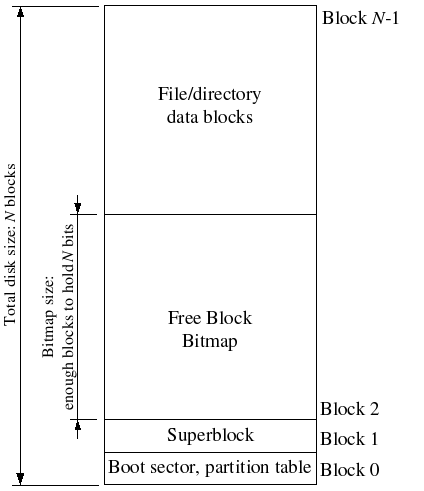
\includegraphics[width=0.6\textwidth]{disk}
\caption{The layout of the file system on the disk. From \cite{lab5}.}
\label{fig:disklayout}
\end{figure}

A file is represented as a \texttt{struct file}, which is stored in its own
block. Such a \texttt{file} struct contains metadata, such as the file name
and size. The struct also has 10 pointers to blocks that hold the raw file
data. If the data cannot fit in 10 blocks, the \texttt{file} struct has a
pointer to a block which holds another 1024 pointers to data blocks. Thus our
file system has a maximum file size of $(10+1024)*4096 = 4235264$ bytes, i.e.,
around 4 MB. The structure of a \texttt{file} is displayed in figure
\ref{fig:filestruct}.

\begin{figure}[h]
\centering
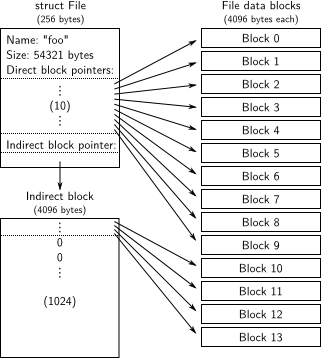
\includegraphics[width=0.6\textwidth]{file}
\caption{The representation of a file. From \cite{lab5}.}
\label{fig:filestruct}
\end{figure}

A folder is represented as a \texttt{struct folder}, which is exactly
identical to a \texttt{struct file}, except that the $10+1024$ block pointers
no longer point to raw data, but to other blocks holding \texttt{file} or
\texttt{folder} structs. There is a type flag which allows distinction between
files and folders.

We used a small script to create a raw disk image with an initialized file
system of the described format. The script let us add files, such as sample
programs, to the file system. We then attached this raw disk to QEMU.



\section{File system daemon}
In accord with exokernel design we let all file system interaction go through
a user-mode process, which we call the file system daemon.

The daemon interacts with the disk using PIO. However a normal user-mode
process cannot use the \texttt{inb} and \texttt{outb} instructions to perform
PIO, so our kernel needs to give the daemon I/O privileges. It does so
by setting a bit in the \texttt{eflags} register while spawning the daemon.

The disk knows nothing of the file system which is stored upon it. The daemon
can merely read a sector of the disk at a time. It is therefore up to the
daemon to implement reading and writing of files and folders according to the
file system specification. We wrote the necessary functions for interacting
with the file system.

The file system daemon spends its time looping, waiting for other processes to
contact it via IPC. Processes can send requests to open, read, write,
and stat files. The IPC details are hidden inside the user-mode C standard
library, giving processes the usual interface with functions such as
\texttt{open}, \texttt{read} and \texttt{write}.

For sake of illustration, the following happens when a process wants to open a
file:
\begin{itemize}
\item The process calls the \texttt{open} library function.
\item The library uses IPC to contact the file system daemon.
\item The daemon reads the superblock to find the block of the root folder.
\item The daemon follows pointers from folder to folder according to the given
path.
\item When the path has been traversed, the daemon has found the block that
contains the \texttt{file} struct.
\item The offset into the disk that holds the \texttt{file} struct is stored
in a file descriptor.
\item File descriptors are numbered; the daemon returns this number as the
result of the IPC call.
\end{itemize}
When the process subsequently reads from the file descriptor, the daemon
uses the pointers in the \texttt{file} struct to find the raw data and return
it via IPC.

We have also implemented a block caching system to improve the efficiency of
the file system daemon. When a block is first read, its contents are stored in
RAM, and subsequent reads do not need to interact with the disk until the
cache entry is invalidated through a write.


\section{Shell}
\label{sec:shell}
To test the interaction between programs and the disk, we implemented a
simplistic shell which allows loading and execution of programs from disk. The
shell allows reads from and writes to the disk through input redirection
(\texttt{<}) and output redirection (\texttt{>}). The shell additionally
supports piping of the output of one program into another program. A small
program, \texttt{cat}, lets the user read files from the disk. A sample interaction
is shown in figure \ref{fig:shellinteraction}.

\begin{figure}[h]
\begin{framed}
\begin{Verbatim}[fontsize=\small]
$ ls
cat
echo
ls
sh
$ echo "Hello, OS." > motd
$ cat motd
"Hello, OS." 
\end{Verbatim}
\end{framed}
\caption{A sample interaction with the shell.}
\label{fig:shellinteraction}
\end{figure}



%%%%% LAB 6 %%%%%
\chapter{Networking}
In this lab we connected our kernel to the internet by writing a network card
driver and adding a TCP/IP stack. We also wrote a small web server to test the
new functionality.

The network card, its kernel driver, and the TCP/IP stack cooperate to make
networking possible. For example, when a process transmits data over the
network, the following steps occur: the data is first delivered to the
TCP/IP stack, which constructs a raw packet. The network card driver then puts
the raw packet in a transmit-queue, which the network card periodically
drains to put the packet on the wire. Receiving data is analogous, with
packets flowing through a receive-queue in the reverse direction. We describe
the details of these components in the following sections.

\section{The network card}
The operating system connects to the network using a network card, whose task it
is to send and receive packets by interacting with the physical layer. QEMU
emulates the Intel e1000 network card, which we therefore targeted. We added
the card to our emulated machine with the \texttt{-net nic,model=e1000} option to
QEMU, which creates a virtual router at IP 10.0.2.2 and assigns the guest an
IP of 10.0.2.15. This let us hardcode the IP address rather than having to
implement a DHCP client or similar.

The e1000 manual \cite{e1000manual} describes in detail the internals of the
card, as well as the steps a driver must take to initialize the card, read
incoming packets, and transmit outgoing packets. 

The e1000 maintains two circular packet queues: a transmit queue and a receive
queue. To send a packet, the kernel adds it to the transmit queue, which the
network card periodically drains. When a packet arrives on the wire, the
network card adds it to the receive queue, which the kernel periodically
drains.

The items in the queues are small descriptor structs, each of which describes
an area of physical memory which can hold a raw packet. The queues are
implemented as arrays, with each queue having a head and tail register to keep
track of the head and tail of the queue.



\section{The network card driver}
We wrote an e1000 network card driver using the information from the manual.
Our kernel uses PIO to scan the PCI bus, iterating over each connected
device until it finds one whose vendor and device ID indicate it being an
e1000 network card. The PCI interface supplies a physical address where the
driver can use MMIO to communicate with the e1000.

With communication possible, the first task of the driver was to initialize
the network card. The driver allocates the arrays that make up the packet
queues and fills these with valid descriptors. It zeroes out the head and tail
registers.

Once our driver has initialized the card, it writes into a register to enable
it. It is then possible to transmit and receive packets. Our driver implements
the code for taking packets from the receive queue and inserting packets into
the transmit queue. User-mode programs have access to this driver
functionality through two system calls, \texttt{sys\_receive} and
\texttt{sys\_transmit}, respectively.

If the transmit queue ever becomes full due to the card draining it too
slowly, it is up to the driver what should happen. For simplicity we have
chosen to simply drop the packet if the queue is full. This is not a problem
because the higher-level protocols are resistant to packet loss. Alternatively
the driver could have blocked, waiting for space in the queue. If, on the
other hand, the receive queue is full, the e1000 is designed to simply drop
further packets.


\section{The network daemon}
With the driver written, our kernel was capable of transmitting and receiving
packets. However most processes only know of the data they wish to send; they
are not capable of constructing packets.

We therefore needed a TCP/IP stack. Allegedly, writing such a network stack
from scratch is an immense task. We therefore used the open-source stack lwIP
(``lightweight IP"). lwIP acts as a black box for our purposes, taking raw data
as input and producing packets as output.

Rather than adding lwIP to the kernel, we embedded it in a network daemon. The
daemon is responsible for managing sockets, just as the file system daemon was
responsible for managing file descriptors. The network daemon takes in
requests to send data via IPC, produces packets, and hands these over to the
operating system via the \texttt{sys\_transmit} system call. Likewise, it
takes in requests to receive data and uses \texttt{sys\_receive}, parses the
resulting packets, and hands over the data to the requesting process.

The IPC communication is hidden away in the C standard library, such that
user-mode programs have access to the familiar \texttt{connect}, \texttt{send}
and \texttt{recv} interface.


\section{Web server}
To test the new functionality, we wrote a simple web server which can serve
files from the file system over HTTP. The web server uses the network daemon
to accept incoming connections and receive HTTP requests. It parses each
request, queries the file system daemon to retrieve the requested file
contents, and uses the network daemon to send back the HTTP response.

We configured QEMU to forward requests at port 80 to the emulated machine. At
this point we were able to point a browser at the machine and be served a
working web page.





%%%%% GRAPHICS LAB %%%%%


\chapter{Graphics}
\label{sec:graphics}

In this lab we implemented a graphical user interface to our operating system.
The end result is that each application is given its own graphical window on
the screen, and the user can interact with applications using the mouse and
keyboard.

The pixels on the screen are represented in a data structure called the Linear
Frame Buffer (LFB), which the kernel must get access to by querying the BIOS.
The kernel can draw pixels on the screen by writing to the LFB. We wrote a
graphics library to draw pixels and more complex shapes.

We then designed a graphics stack, which involved deciding how input and
output events should flow through the system from kernel to user application.
After reading about how graphics work in other systems \cite{graphicsstack,
windowingsystem, xwindowsystem} we decided upon a design with a central
display server, which is responsible for rendering all of the screen and which
acts as an intermediary for input and output events.

Finally we added a few sample graphical applications to demonstrate the new
features, including a paint application and a terminal emulator.


\section{Mapping the Linear Frame Buffer}
To initialize graphics, the operating system must query the BIOS to select a
video mode, which is a description of the width, height and depth of the
screen. Once a video mode is selected, the BIOS maps a crucial data structure
into memory, which is called the Linear Frame Buffer (LFB).

The LFB represents the pixels of the screen; it can be thought of as a
two-dimensional array, where each value is a 32-bit integer representing the
RGB value of a pixel on the screen. Thus to write a pixel to the screen, the
kernel must simply calculate the correct offset into the LFB and write a
32-bit integer there.

The kernel queries the BIOS to set a video mode using the
\texttt{int 0x10} instruction. This transfers execution to the BIOS. However
since the BIOS is written as 16-bit real mode code, our kernel must switch the
processor back to 16-bit real mode before it can issue the interrupt.
We therefore wrote assembly code which switches the processor mode,
queries the BIOS to enumerate the valid video modes, and selects one with a
satisfactory resolution.

At this point our kernel was able to draw pixels on the screen by writing to
the LFB. However the kernel lacked the ability to draw more complex shapes.


\section{Graphics library}
We used the ability to draw a single pixel as a building block, writing
functions that can draw more complex shapes, such as straight lines,
rectangles, and windows. We also implemented font rendering.

Since this functionality is needed by many different applications, we put it
inside a graphics library which is available to user space applications.


\section{Graphics stack design}
To implement a user interface, we needed to decide how input and output events
should flow through the system. When a mouse click or key press occurs, the
kernel receives an interrupt. How should this event arrive at a user space
application, and which should it be? Should a user space application render
its own pixels? If so, how does it know which parts of the LFB it can write to
without clashing with other applications? 

After considering these questions and reading about how other operating
systems render graphics, we decided to let all events flow through a central
privileged process, called the display server. 

The display server takes input events from the kernel and delivers them to the
target application. Each application has a canvas. The display server takes
output events from the applications, in the form of changes to the canvas, and
writes the changes to the LFB.

Each graphical application waits to receive events from the display server in
an event loop. The application can make changes to its canvas on the basis of
an event occurring.

The kernel keeps a queue for input events. When raw input packets arrive from
the mouse or keyboard, a driver handles these packets by putting them into an
event queue. The display server periodically drains this queue through a
system call, forwarding the events.

Figure \ref{graphicslayout} shows the different components in the graphics
stack and how they interact. 
\begin{figure}[h]
\centering
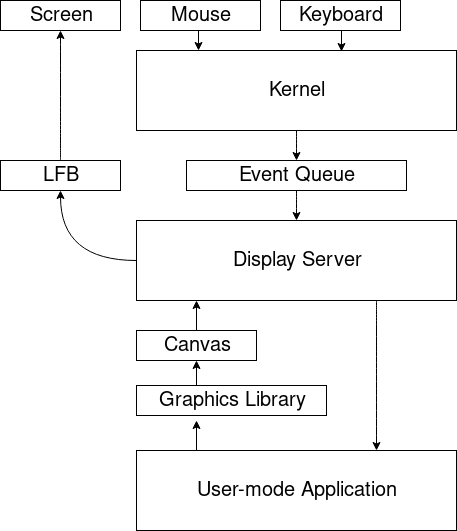
\includegraphics[width=0.6\textwidth]{flow-diagram2.png}
\caption{The graphics stack components and their interaction.}
\label{graphicslayout}
\end{figure}

The following sequence of events exemplifies the flow of events through the
graphics stack:
\begin{itemize}
\item The user presses the 'A' key.
\item The keyboard generates an interrupt to signal to the kernel that input
is available.
\item The kernel keyboard driver reads the pressed key using PIO.
\item The driver puts the event into the events queue.
\item The display server eventually drains the events queue and finds the key
press event.
\item The display server finds that the terminal application is active and
therefore forwards the event to it using IPC.
\item The terminal application receives the event and adds the 'A' to a buffer
which holds the current input of the user. This buffer will eventually be used
to run a command once the user presses the enter key.
\item The terminal application also wants to display the 'A' on the screen, so
that the user can see what is written so far. The application therefore asks
the graphics library to render an 'A' on its canvas using the default font.
\item The display server writes the pixels from the canvas into the part of the
LFB that contains the application window.
\item The user sees the 'A' appear on screen.
\end{itemize}
We describe the details of how we have implemented the display server in the
following section.


\section{The display server}
Various events must be performed periodically by the display server: it must
drain input events from the kernel and deliver these to applications, and it
must render the canvases of applications by writing to the LFB. We show the
code for the main loop of the display server in figure \ref{displayserver}.
\begin{figure}[h]
\begin{framed}
\begin{Verbatim}[fontsize=\small]
while (1) {
	// drain input events from the kernel 
	// and decide how to handle them
	process_events();

	// deliver events to targeted applications
	transmit_events();

	// draw the desktop background
	draw_background();

	// draw each application in the correct order
	draw_applications();

	// finally, draw the cursor on top
	draw_cursor();
	
	// write the changes to the LFB
	refresh_screen();
}
\end{Verbatim}
\end{framed}
\caption{The main loop of the display server.}
\label{displayserver}
\end{figure}

The display server is responsible for writing the pixels of every application
into the LFB. For efficiency the display server bypasses the kernel and writes
directly to the LFB, which is accomplished by mapping the LFB into the address
space of the display server using a new system call, \texttt{sys\_map\_lfb}.

The display server is responsible for spawning every other graphical
application and assigning the application a portion of the screen. When
spawning an application, an area of shared memory is set up through IPC.
This memory is the canvas of the application. The application can write pixels
into the canvas, and the display server will periodically read the canvas and
write any changes to the LFB. 

The display server determines the ordering of applications along the z-axis,
drawing the pixels of the topmost application last. It also determines which
application is currently active and directs key presses only to it.

It is highly important that the display server is efficient; if it runs too
slowly, the system will have a low frame rate, with interaction feeling
choppy. We had to carefully optimize the code for the display server before we
got an acceptable frame rate inside QEMU.

We wrote a mouse driver for a PS/2 mouse which reads data packets from the
mouse through PIO \cite{mouseinput}. These data packets are generated whenever
the mouse is moved. They only contain delta x- and y-coordinates, which means
that the concept of a cursor only exists inside the display server.


\section{Sample graphical applications}
To test our design and implementation we have written two simple graphical
applications: a paint program and a terminal emulator. 

The paint program allows the user to click its canvas, drawing a square as a
result.

The terminal emulator accepts keyboard input. It renders the input as the user
types it. When the enter key is pressed, the terminal emulator forwards the
input to a non-graphical process running the simple shell which we described
in section \ref{sec:shell}. The output of this shell process is displayed to
the user inside the terminal emulator.

An interaction with the two applications is displayed in figure \ref{desktop}.
\begin{figure}[h]
\centering
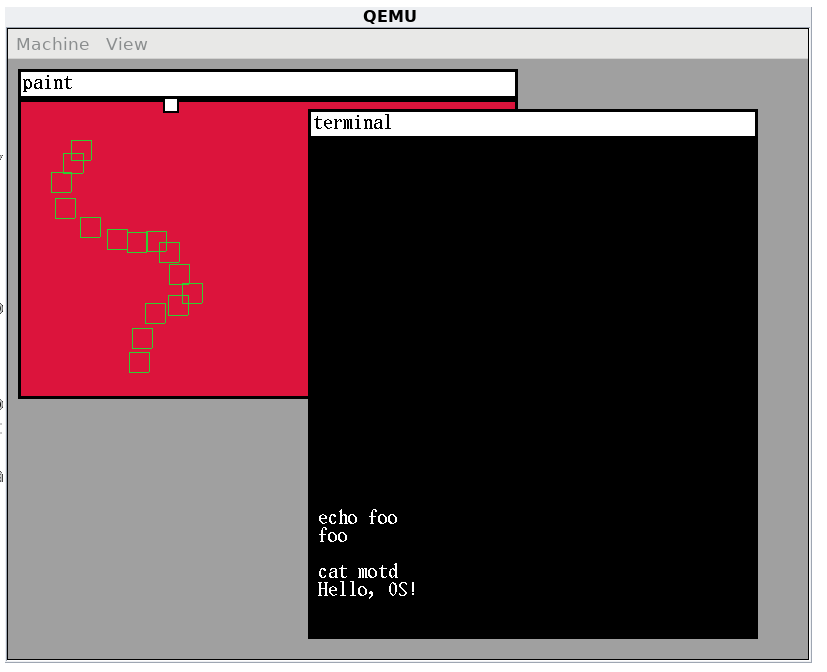
\includegraphics[width=0.8\textwidth]{interaction}
\caption{Interaction with two graphical applications.}
\label{desktop}
\end{figure}








%%%%% HARDWARE LAB %%%%%
\chapter{Hardware}
In this lab we modified our operating system to let it run on real hardware
rather than the QEMU emulator.

The main cause of difficulty was that our chosen hardware differed from the
hardware emulated by QEMU. Additionally, there are aspects of a machine that
QEMU does not emulate faithfully for efficiency reasons, but which matter when
writing an operating system. This caused latent bugs to surface once we
switched to real hardware.

In the following sections we describe the steps we took to get our operating
system running on our machine of choice, a Packard Bell Dot S netbook
\cite{netbook}.


\section{Booting from USB}
To boot our operating system we had to write its raw disk image to a bootable
medium, such as a hard drive or a USB drive. We preferred to boot from a USB
drive, since the hard drive would require either cable access or booting into
a different operating system to transfer the image, which would be slow and
tedious.

When we supplied our raw disk image to QEMU it booted as expected. We
therefore expected that the same would happen when we transferred the image to
a USB drive and inserted it into the netbook. However the USB was not
recognized as a bootable medium. 

The reason turns out to be historical \cite{bootingfromusb}: when USB
technology was new, there was disagreement between manufacturers on whether a
USB drive should be a raw storage drive or a bootable medium. Initially the
user could decide through a BIOS setting, but for usability reasons,
manufacturers eventually opted to use heuristics to detect whether a USB is
bootable or not. 

These heuristics are based on data structures called the Master Boot Record
(MBR) and BIOS Parameter Block (BPB). Both the MBR and BPB must be present in
the first sector of a USB drive, otherwise most machines will assume that the
drive is merely for data storage. 

Once we added a valid MBR and BPB to our boot loader, the USB was recognized
as bootable and the boot loader executed. Unfortunately it got stuck. The
problem was that the boot loader was programmed to load the operating system
from a hard drive connected through an ATA cable.

We realized that to continue, we would have to rewrite our boot loader to
support loading from USB. However the boot loader is constrained to 512 bytes,
since the BIOS loads it from the first sector of the drive. Writing code that
can load from both USB and ATA drives in 512 bytes seemed difficult.

In the end we replaced our boot loader with a better one, namely GRUB, which
supports booting from various hard drive types, USB, and even an ethernet
connection. 

We had to modify our file system to incorporate GRUB; the file system assumes
that the boot loader will fit into the first 512 bytes, with the superblock
residing in the following sector. Since GRUB uses multiple stages it needs
much more space. We therefore had to modify our file system such that the
first 32 MB are reserved for GRUB, and the superblock resides thereafter.

After integrating GRUB into the project we were finally able to boot directly
from USB and have kernel code loaded. Unfortunately the scheduler seemed
broken; it was unable to switch in new processes.



\section{Finding the LAPIC}
Debugging showed that timer interrupts were not being generated, which
prevented the scheduler from preempting the running process. The LAPIC is
used to generate these timer interrupts.

In section \ref{sec:mpconfig} we described how our kernel uses the so-called
mpconfig method to find the LAPIC; that is, it looks for an MP
configuration table in memory to find the physical address of the LAPIC. This
address is used to communicate with the LAPIC, asking it to generate timer
interrupts. However our kernel failed to find these configuration tables. They
were simply not present in the memory of the netbook.

It turns out that the mpconfig method is outdated and unsupported by
modern hardware. We therefore had to implement a different way to find the
LAPIC.

We leave out the details of the method, but in essence newer machines contain
so-called ACPI tables \cite{symm}. One of these is the APIC table, which
contains the physical address of the LAPIC. The ACPI tables can be found by
scanning a region of memory for a data structure called the RSDP \cite{rsdp},
which points at another data structure, the RSDT, which finally points at the
ACPI tables.

After implementing this finding and parsing of ACPI tables, the kernel was
able to discover the LAPIC and timer interrupts were generated, letting the
scheduler work as intended.


\section{Latent bugs}
Our kernel was behaving oddly; modifying a PTE seemed to have no effect.
After the modification, writing to memory at the virtual address still
affected memory at the old physical address rather than the new one.

Since this seemed to be a caching issue, we realized that it was likely
related to the TLB. Eventually we learned that the \texttt{invlpg}
instruction must be used to invalidate a TLB entry after a PTE has
been modified. Otherwise the outdated TLB entry will continue to be used
until it is evicted from the cache.

Interestingly, this bug never surfaced while running the kernel in QEMU. We
assume that QEMU does not faithfully emulate the TLB for performance
reasons.\footnote{VirtualBox behaved similarly to QEMU; we therefore believe
that this quirk can be used as a means to detect virtualization/emulation.}

After fixing the page table bug the machine successfully booted into a
graphical interface. However the mouse behaved oddly, jumping around when
moved.


The PS/2 mouse driver we wrote during the graphics lab was at fault; the
driver uses PIO to read from the mouse. Before each \texttt{inb}
instruction, it is necessary to wait for the mouse to signal that it has sent
another byte of data. The driver did not do this. However in QEMU these waits
were not necessary; thus this was another instance of QEMU not emulating
hardware perfectly. We inserted the necessary delays in the mouse driver.


With all the changes and fixes described so far, our operating system finally
ran on the netbook and behaved as expected. 

\section{The development process}
The bugs and issues we have described seem rather obvious when explained in
hindsight. But in practice, debugging a live system without a debugger was
tricky and time-consuming. This was aggravated by there being a sizable delay
between writing code and getting feedback from the machine, caused by us
having to write the kernel image to a USB drive and switch it between
machines for every code change.

For the page table bug, we only observed that processes behaved oddly when
writing to memory. It took a lot of time and print statements before we
realized the root cause of the problem. The other bugs and issues were
similar.

In conclusion, there are significant advantages to developing an operating
system on an emulator rather than a physical machine, despite emulators not
being entirely accurate. Moving the operating system to real hardware was a
time-consuming but not conceptually difficult process; the main task was
supporting different hardware types and standards.




% \chapter{Future work}
% we could talk about future work.
% - security: ASLR, probably many other things (it's not even a multi-user
% system yet)
% - capabilities?
% - basic programs like an editor, browser, etc.
% - better windowing system (faster algorithms, better fonts, z-coordinate..)
% - could get a better scheduler
% - could have true kernel concurrency
% - better file system (timestamps, ...)
% - more efficient display server
% - more drivers.... e.g. network cards.


% I moved this paragraph here from the scheduler.

% Our scheduler has much room for improval. Round-robin scheduling is not as
% performant as more advanced algorithms. Additionally, it does not allow
% adjustment of process priorities. Scheduling being a linear-time operation is
% potentially worrying. 
% 
% A final issue is that the time slice assigned to each process is always of the
% same duration. It would be useful to assign shorter time slices and more
% frequent schedulings to processes which need to feel responsive (such as
% graphics-based processes introduced later) and longer time slices to processes
% that perform heavy computations.

\chapter{Conclusion}
By writing an operating system from scratch we have gained a deep
understanding of the many tasks that it must perform. 


% We have understood the boot process and the importance of a good boot loader.
We have implemented the necessary infrastructure to run a user-mode process;
this included physical page management, page table initialization, program
loading, context switching, interrupt handling, and much else besides. We have
extended this infrastructure to support true concurrency, efficient forking,
and process interaction through an IPC mechanism. We also implemented a custom
file system and networking. Altogether, this infrastructure provides all the
necessary primitives to build complex applications that can run in user space.

By designing and implementing a graphical user interface for our system we
have additionally seen how a graphics stack works from the bottom up. The end
result is that each application may run in a separate graphical window,
allowing interaction through the mouse and keyboard.

We have seen techniques that allowed us to move functionality from the kernel
to user space according to exokernel principles. Examples of this include the
network stack, the display server, and the file system code. We have also
gained experience writing drivers for various devices, including a networking
card and a PS/2 mouse.

By moving our operating system to a real machine rather than an emulator we
have seen the advantages emulators bring to kernel development. We have also
become more aware of the limitations of emulators.

Throughout this process we have been repeatedly surprised by the scope of
services that an operating system must provide, and which we previously took
entirely for granted.


\bibliographystyle{unsrt}
\bibliography{references}

\end{document}

